\documentclass[11pt,titlepage,dvipdfmx,twoside]{jarticle}
\linespread{1.1}

\usepackage{amsfonts}
\usepackage{amssymb}
\usepackage{amsmath}
\usepackage{amsthm}
\newtheorem{theorem}{Theorem}
\newtheorem{lemma}[theorem]{Lemma}
\usepackage{enumitem}
\usepackage{geometry}
\geometry{left=2.5cm,right=2.5cm,top=2.5cm,bottom=2.5cm}

\usepackage{algorithm}  
\usepackage{algorithmic}  
\renewcommand{\algorithmicrequire}{\textbf{Input:}} 
\renewcommand{\algorithmicensure}{\textbf{Output:}}
\renewcommand{\algorithmicforall}{\textbf{for each}}

\usepackage{mathtools}
\usepackage{comment}
\usepackage[dvipdfmx]{graphicx}
\usepackage{float}
\usepackage{framed}
\usepackage{graphicx}
\usepackage{subcaption}
\usepackage{listings}
\usepackage{color}
\usepackage{url}
 
\definecolor{codegreen}{rgb}{0,0.6,0}
\definecolor{codegray}{rgb}{0.5,0.5,0.5}
\definecolor{codepurple}{rgb}{0.58,0,0.82}
\definecolor{backcolour}{rgb}{0.95,0.95,0.92}
 

\newcommand{\dist}{\mathrm{dist}}

\title{\Huge{学習後のニューラルネットワークに基づくMILP (Acyclic Branch-height)の構築方法}}

\begin{document}

% The following makeatletter must be after begin{document}
\makeatletter 
\let\c@lstlisting\c@figure
\makeatother

\西暦
\date{\today}

\maketitle

% \cleardoublepage

\thispagestyle{empty}
\tableofcontents
\clearpage

\pagenumbering{arabic}

\section{概要}
\label{sec:Intro}
この冊子は,学習後のニューラルネットワークを用いて,特定の化学活性を有する化合物の構造情報を計算する
混合整数計画問題(MILP)を構築する方法について説明したものである.

化合物の構造を数値化した特徴ベクトルと化合物の性質を表す値である活性値の組をもとに学習させたニューラルネットワークを用いて,
所望の活性値を有するような化合物の特徴ベクトルを計算するMILPを構築する.
この冊子では,このMILPの構築方法とPythonを用いたプログラムの実装内容について説明する.

また,このフォルダにはこの冊子以外に以下のフォルダやファイルが含まれている.

\begin{itemize}

\item フォルダsource\_code\\
特徴ベクトルを計算するMILPをPythonを用いて実装したプログラムが含まれているフォルダである.
\begin{itemize}
\item {\tt infer\_acyclic\_graphs.py}\\
MILPによる計算を実行するプログラムである.
このプログラムの使い方は第\ref{sec:Exp}節を参照すること.
\item {\tt ann\_inverter.py}\\
ANNの逆問題を定式化したMILPをPythonで実装したソースコードである.
このプログラムの説明は第\ref{sec:Code}節を参照すること.
\item {\tt acyclic\_graphs\_MILP.py}\\
計算した特徴ベクトルを満たす化合物が存在するための必要十分条件を実装したソースコードである.
このプログラムの説明は第\ref{sec:Code}節を参照すること.
% \item {\tt \_\_init\_\_.py}\\
% プログラムをPythonによって実行するために必要な空のファイルである.
\end{itemize}

\item {フォルダ}test\_files\\
ニューラルネットワークによる学習のデータが含まれているフォルダである.
\begin{itemize}
\item {\tt rt\_biases.txt}\\
化学活性retention timeのデータを用いて学習させたニューラルネットワークのバイアスのデータが含まれているテキストファイルである.
フォーマットについては第\ref{sec:InOut}節を参照すること.
また,このデータを用いて実験を行なった計算例を第\ref{sec:Exp}節に示す.
\item {\tt rt\_weights.txt}\\
化学活性retention timeのデータを用いて学習させたニューラルネットワークのウェイトのデータが含まれているテキストファイルである.
フォーマットについては第\ref{sec:InOut}節を参照すること.
また,このデータを用いて実験を行なった計算例を第\ref{sec:Exp}節に示す.
\item {\tt rt\_fv4\_new.txt}\\
化学活性retention timeのデータと特徴ベクトルのデータが含まれているテキストファイルである.
フォーマットについては第\ref{sec:InOut}節を参照すること.
また,このデータを用いて実験を行なった計算例を第\ref{sec:Exp}節に示す.
\item {\tt rt\_fv4\_new\_max.txt}\\
化学活性retention timeのデータと特徴ベクトルのデータが含まれている各要素の最大値である.
AD制約式の上界値が含まれるファイルである.
\item {\tt rt\_fv4\_new\_min.txt}\\
化学活性retention timeのデータと特徴ベクトルのデータが含まれている各要素の最小値である.
AD制約式の下界値が含まれるファイルである.
\end{itemize}

% \item MILP定式化の正当性.pdf\\
% 化合物を推定するためのMILPの定式化の正当性を説明した資料である.
% 
% \item 木状化合物推定(隣接行列法).pdf\\
% 木状化合物を推定する方法を紹介した論文である.

\end{itemize}

次に,この冊子の構成について説明する.
第\ref{sec:Pre}節では,この冊子およびプログラム内で使用している用語について説明する.
第\ref{sec:InOut}節では,プログラムの入力と出力について説明する.
この節では,プログラムの入力情報と出力情報を具体例を用いて説明する.
また,実際に計算機に入力する際に使用するデータ形式や,プログラム実行後に出力されるデータの形式も説明する.
第\ref{sec:Exp}節では,プログラムの計算例について説明する.
この節では具体例を用いて,実際に計算機上でプログラムを実行した結果を紹介する.

以上のような流れで,プログラムの実行内容について説明していく.

% \newpage

\section{用語の説明}
\label{sec:Pre}
この節では,冊子とプログラムの中で使用する用語について説明する.
この節で紹介した用語をもとに冊子とプログラム内の説明を行っていく.

\begin{itemize}
\item 特徴ベクトル\\
特徴ベクトルとは,化合物の構造から予測する活性と関係のありそうな特徴をいくつか抽出・算出し,それらを成分としたベクトルである.
このプログラムでは化合物の特徴ベクトルから,その化合物が持つ活性を予測する.

\item ニューラルネットワーク \\
ニューラルネットワークとは,機械学習の手法の一つであり,入力されたベクトルをもとに目的とする値を予測する手法である.
この冊子では,化合物の特徴ベクトルを入力した際に,その化合物が持つ活性値の予測値を出力するようなニューラルネットワークを構築する.

\item 入力層,中間層,出力層\\
ニューラルネットワークはいくつかの層で構成されている.
まず,特徴ベクトルが入力される層が入力層である.
入力層は特徴ベクトルの要素数と同じ数のノードで構成されている.
次に,予測値の計算を段階的に行なっていくのが中間層である.
中間層は前の層から入力された値をもとに計算を行い,次の層に出力する.
最後に,予測値を出力するのが出力層である.
この冊子では一つの活性値を出力するため,出力層は一つのノードで構成されている.
ある層に含まれるノードは,次の層の全てのノードに接続されている構造を持っている.

\item ウェイト(重み)\\
ニューラルネットワークに含まれているノード間を接続している枝はそれぞれ値を持っており,その値をウェイトと呼ぶ.
ニューラルネットワークは,既知の特徴ベクトルと活性値のペアをデータセットとし,それらを関連付けるために学習を行う.
ニューラルネットワークの学習によって,ウェイトが決定される.
この冊子では,学習後のニューラルネットワークのウェイトを取り出す方法について説明する.

\item バイアス\\
中間層と出力層に含まれているノードはそれぞれ値を持っており,その値をバイアスと呼ぶ.
ウェイトと同様に,ニューラルネットワークの学習によって,バイアスの値が決定される.
この冊子では,学習後のニューラルネットワークのバイアスを取り出す方法についても説明する.

\item 活性化関数\\
ニューラルネットワークには,予測値を計算するために用いられる活性化関数が定められている.
ニューラルネットワークの各ノードでは,入力された値を活性化関数に入力し,その関数の出力値をそのノードの出力値としたて計算を行なっていく.
この冊子ではRectified Linear Unit関数(ReLU)を活性化関数として扱っていく.
% ReLU関数についての詳細は第\ref{sec:MILP}節を参照すること.
%https://scikit-learn.org/stable/modules/generated/sklearn.neural\_network.MLPRegressor.html

\item 混合整数計画問題(MILP)\\
一部の決定変数が整数であり,制約式や目的関数が線形の式で表されている問題を混合整数計画問題(MILP)と呼ぶ.
詳細については参考文献~\cite{LP}を参照すること.

%\item 化学グラフ\\
%化学グラフは節点集合と枝集合の組で構成されており,化合物の平面構造を表すものである.
%各節点には原子の種類が割り当てられており,各枝には結合の多重度が割り当てられている.
%この冊子では水素原子が省略された化学グラフを扱っていく.

\item グラフ\\
点の有限集合と点対である辺の有限集合によって定義される構造をグラフと呼ぶ.
この冊子では辺の方向を考慮する有向グラフを扱う.
詳細については参考文献~\cite{graph}を参照すること.

\item 有向木\\
長さ1以上の閉路を持たず連結である有向グラフを有向木と呼ぶ.
有向木において枝$(u,v)$が存在するとき,$u$は$v$の親,$v$を$u$の子と呼ぶ.
詳細については参考文献~\cite{graph}を参照すること.


\item スキーム木\\
すべての対応グラフが部分グラフになれるの木構造のグラフ.

\end{itemize}

% \newpage

\section{プログラムの入力と出力}
\label{sec:InOut}

この節では,プログラムの入力と出力について説明する.
\ref{sec:section3_1}節では,プログラムの入力情報について具体例を用いて説明する.
\ref{sec:section3_2}節では,計算機上で入力する際のデータ形式について説明する.
\ref{sec:section3_3}節では,プログラムの出力情報について具体例を用いて説明する.
\ref{sec:section3_4}節では,計算機上でプログラムを実行した際に出力されるデータ形式について説明する.

\subsection{プログラムの入力}
\label{sec:section3_1}

この節では,プログラムの入力情報について説明する.
このプログラムでは計算で使用する三つのテキストファイル,
スキーム木が満たすべき数値データと,
出力される化合物が満たすべき数値データを入力とする.

まず,入力する三つのテキストファイルについて説明する.

一つ目は,特徴ベクトルを入力した際に目的とする化学活性の活性値を予測する
ニューラルネットワークのウェイトのデータが含まれているテキストファイルである.

二つ目は,特徴ベクトルを入力した際に目的とする化学活性の活性値を予測する
ニューラルネットワークのバイアスのデータが含まれているテキストファイルである.

三つ目は,目的とする化学活性の活性値を予測するニューラルネットワークを学習させるために
用いた特徴ベクトルのデータが含まれているテキストファイルである.

次に,スキーム木が満たすべき三つの数値データ$k^\ast, {\rm bn}_{k^\ast}, {\rm bh}_{k^\ast}$を入力する.

最後にに,化合物が満たすべき四つの数値データを説明する.
入力する四つの数値は,化合物が持つ原子数$n^{\ast}$,求められる活性値tv$^\ast$, 化合物の構造グラフの最大次数$d_{max}$と直径dia$^\ast$である.

このプログラムでは,入力された三つのテキストファイルと
入力スキーム木においてのグラフを持つ出力される化合物が満たすべき数値データをもとに,
入力した活性値に近い値を持つような特徴ベクトルを算出する.

\bigskip

\subsection{入力データの形式}
\label{sec:section3_2}

この説では,計算機上で入力する際のデータ形式について説明する.
\ref{sec:section3_1}節で説明した三つのテキストファイルの形式について具体例を用いて説明する.

このプログラムでは学習後のニューラルネットワークを用いて特徴ベクトルの計算を行う.
その具体例が図~\ref{fig:sample}である.
図\ref{fig:sample}の学習後のニューラルネットワークには,ウェイトとバイアスが記入されている.
この情報を二つのテキストファイルで表現する.

\begin{figure}[H]
  \centering
  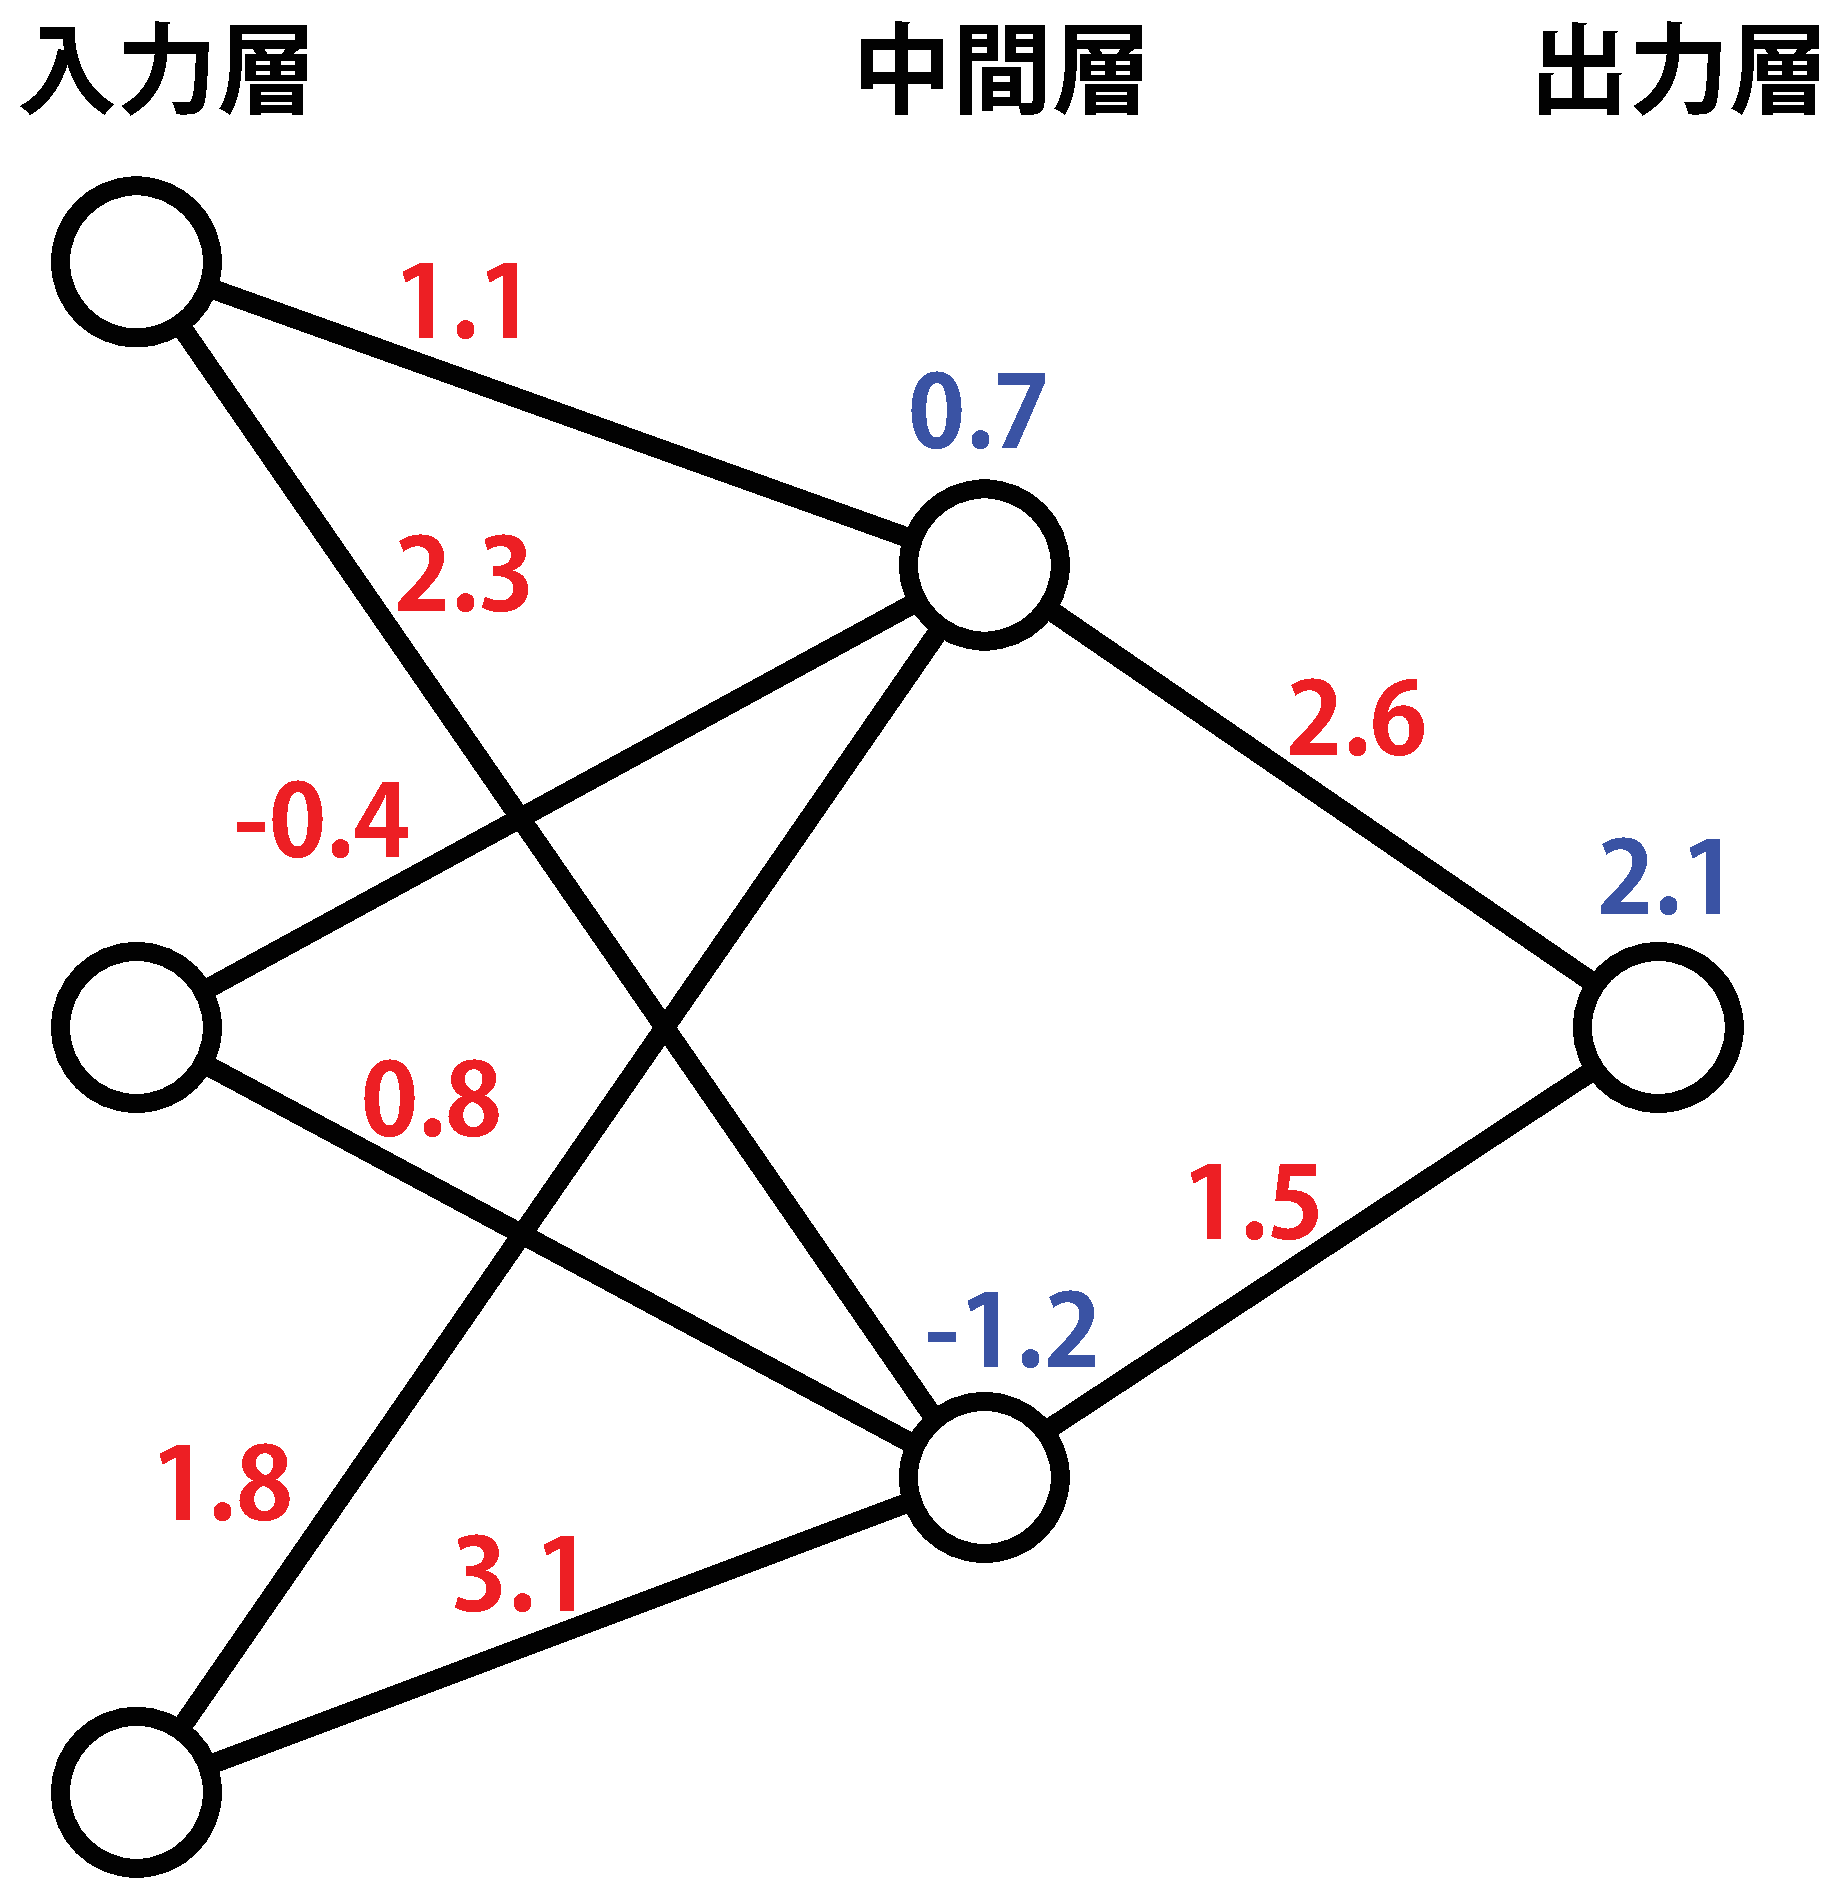
\includegraphics[width=0.4 \columnwidth]{./fig/ANN_sample_jp}
  \caption{学習後のニューラルネットワークの具体例.赤色の数値がウェイト,青色の数値がバイアスを表している.}
  \label{fig:sample}
\end{figure}

学習後のニューラルネットワークのウェイトとバイアスの情報は二つのテキストファイルとして出力される.

まず一つ目はウェイトのデータが含まれたテキストファイルである.
このテキストファイルでは一行目にニューラルネットワークの構造が記入されている.
入力層,中間層,出力層のノード数がそれぞれ記入されている.
二行目以降はウェイトのデータが記入されている.
各行には入力層のノードから次の中間層の全てのノードへの枝のウェイトが記入されている.
続いて,中間層から出力層への枝のウェイトが記入されている.
図~\ref{fig:sample}のウェイトのデータを記入したテキストファイルは以下のようになる.

\bigskip

\begin{oframed}
{\bf ウェイトのデータ形式}\\\\
%\bigskip\bigskip
3 2 1\\
1.1 2.3\\
-0.4 0.8\\
1.8 3.1\\
2.6\\
1.5\\
\end{oframed}

\bigskip

二つ目はバイアスのデータが含まれたテキストファイルである.
各行にバイアスの値が記入されている.
記入されている順番は,入力層の一つ目のノードから最後のノード,中間層の一つ目のノードから最後のノード,出力層のノードである.
図~\ref{fig:sample}のバイアスのデータを記入したテキストファイルは以下のようになる.

\bigskip

\begin{oframed}
{\bf バイアスのデータ形式}\\\\
%\bigskip\bigskip
0.7\\
-1.2\\
2.1\\
\end{oframed}

\bigskip

最後に,特徴ベクトルのデータが含まれたテキストファイルの形式について説明する.
このテキストファイルでは,一行目に特徴ベクトルの構成要素が記入されている.
二行目以降の各行に特徴ベクトルの数値データが記入されている.
このテキストファイルの具体例を以下に示す.

\bigskip

\begin{oframed}
{\bf 特徴ベクトルのデータ形式}\\\\
%\bigskip\bigskip
CID,n,M,C,O,H,C1O,C2O,C1C,C2C,\#degree1,\#degree2,\#degree3,\#degree4,\#degree5,\\
\#degree6,\#double\_bond,\#triple\_bond,Diameter,bc\_121,bc\_122,bc\_123,bc\_131,
bc\_132, \\bc\_141,bc\_221,bc\_222,bc\_223,bc\_231,bc\_232,bc\_241,bc\_331,bc\_332,bc\_341,bc\_441,2-branch\_height,2-branch\_number\\
7778,13,126.154,11,2,20,2,1,8,1,4,7,2,0,0,0,2,0,0.769231,0,1,0,3,0,0,5,0,0,2,1,0,0,0,0,0,1,2
\\
86749,11,123.636,10,1,20,1,0,8,1,5,4,1,1,0,0,1,0,0.636364,1,0,0,2,0,2,2,0,0,0,1,2,0,0,0,0,1,2
\\
5282109,13,126.154,11,2,18,2,1,7,2,4,7,2,0,0,0,3,0,0.769231,0,1,0,3,0,0,5,0,0,1,2,0,0,0,0,0,1,2
\\
5319723,11,123.636,10,1,16,1,0,6,3,4,5,2,0,0,0,3,0,0.727273,1,1,0,1,1,0,2,0,0,3,1,0,0,0,0,0,1,2
\\
\hspace{5mm}\vdots
\\
\hspace{5mm}\vdots

\end{oframed}

\bigskip



\subsection{プログラムの出力}
\label{sec:section3_3}

この節では,プログラムの出力情報について説明する.
このプログラムでは,与えられた活性値を満たすような特徴ベクトルが存在する場合は
その特徴ベクトルを出力する.
そなような特徴ベクトルが存在しない場合は,存在しないと出力する.
次の節で出力結果の形式について説明する.

\subsection{出力データの形式}
\label{sec:section3_4}

この説では,計算機上でプログラムを実行した際に出力されるデータ形式について説明する.


まず特徴ベクトルのそれぞれの特徴量が各行に表示される.
次に,化学グラフの情報が表示される.
各節点が対応する原子が表示される.
それぞれの節点には番号が割り振られている.
そして,各節点の隣接リストが表示される.
リストに含まれる節点番号の原子に結合が存在することを表しており,括弧内の値は結合の多重度を表している.
出力結果の具体例を以下に示す.

\bigskip

\begin{oframed}
{\bf ターミナル上の出力結果のデータ形式}\\\\
%\bigskip\bigskip
Status:Optimal \\ 
Initializing Time: 3.8026208877563477 \\ 
Solving Time: 20.04114603996277

\end{oframed}

さらに,ターゲット値及び他の引数に応じての名前が変わる{\tt sdf}ファイルが結果として作ります.
このファイルは世界中水準の{\tt sdf}フォーマットで一つのグラフを格納しています.



\section{プログラムの実行と計算例}
\label{sec:Exp}

この節ではプログラムの実行例を説明する.
ここではプログラム{\tt infer\_acyclic\_graphs.py}の実行方法と結果の具体例を示す.

\subsection{環境確認}
MacBook Air (13-inch, 2017)において:\\
~~~~プロセッサー1.8 GHz Intel Core i5\\
~~~~メモリー 8 GB 1600 MHz DDR3\\
~~~~起動ディスク Macintosh HD\\
~~~~グラフィックス Intel HD Graphics 6000 1536 MB\\
のターミナルバージョン2.9.5 (421.2)でコンパイルすれば問題ないと考えられる。


\subsection{実行方法}
\label{sec:Exp_1}

まず,ターミナル上でディレクトリをフォルダsource\_codeに変更する.
このプログラムを実行するためには,ターミナル上で以下のコマンドを実行する.\\

{\tt python3 infer\_acyclic\_graphs.py target value 
$n^\ast$ ${\rm dia}^\ast$ $k^\ast$ $d_{\max}$ bn$_{k^\ast}$  bh$_{k^\ast}$ solver\_type property}\\

ここで, solver\_type=1の時,ソルバーとしてCPLEXが使われる. solver\_type=2の時,ソルバーとしてCoin-ORが使われる.
例えば,
target value=1900 $n^\ast$=15 ${\rm dia}^\ast$=10 $k^\ast$=2 $d_{\max}$=3 bn$_{k^\ast}$=3 bh$_{k^\ast}$=2 solver\_type=1  
propertyがretention timeとすれば,コマンドが以下のようになる.\\

{\tt python3 infer\_acyclic\_graphs.py 1900 15 10 2 3 3 2 1 rt}\\

このコマンドを実行すると計算が実行され,計算結果が出力される.


\begin{oframed}
{\bf 出力データの形式}\\\\
%\bigskip\bigskip
{\tt 2\\
C 120 4 5 8\\
O 160 2 2 0\\
3\\
C C 2 0 3\\
C O 1 4 0\\
C C 1 2 5\\
0 6\\
4 1\\
3 1\\
0 0\\
10\\
3\\
1 2 1 0 1\\
1 2 2 0 0\\
1 2 3 0 0\\
1 3 1 0 2\\
1 3 2 0 3\\
1 4 1 0 0\\
2 2 1 2 0\\
2 2 2 0 0\\
2 2 3 0 0\\
2 3 1 4 1\\
2 3 2 0 0\\
2 4 1 0 0\\
3 3 1 0 1\\
3 3 2 0 0\\
3 4 1 0 0\\
4 4 1 0 0\\}
\end{oframed}


この具体例を用いて,各行の内容を説明する.
数値例とそれぞれの内容の対応を表~\ref{tab:InputFormat}に示す.

\bigskip
\begin{table}[H]
\begin{center} \caption{入力するテキストファイルの読み方}
\label{tab:InputFormat}
  \begin{tabular}{l|l}
  数値例 & 内容\\ \hline \hline
{\tt  2} & 原子の種類\\ \hline
{\tt  C 120 4 5 8} & 原子のシンボル,質量の十倍,価数,原子の内部節点数,原子の外部節点数\\
{\tt  O 160 2 2 0} & \\ \hline
{\tt  3} & 原子結合の種類 \\ \hline
{\tt  C C 2 0 3} & \\
{\tt  C O 1 4 0} &  原子結合(原子,原子,多重度),内部原子結合の数,外部原子結合の数 \\
{\tt  C C 1 2 5} & \\ \hline
{\tt  0 6} & 度数が1の内部節点数,度数が1の外部節点数 \\ 
{\tt  4 1} & 度数が2の内部節点数,度数が2の外部節点数 \\
{\tt  3 1} & 度数が3の内部節点数,度数が3の外部節点数 \\
{\tt  0 0} & 度数が4の内部節点数,度数が4の外部節点数 \\ \hline
{\tt  10} & 直径 \\ \hline
{\tt  3} & 度数の上限 \\ \hline
{\tt  1 2 1 0 1} & \\
{\tt  1 2 2 0 0} & \\
{\tt  1 2 3 0 0} & \\
{\tt  1 3 1 0 2} & \\
{\tt  1 3 2 0 3} & \\
{\tt  1 4 1 0 0} & \\
{\tt  2 2 1 2 0} & 度数結合(度数,度数,多重度),内部度数結合の数,外部度数結合の数 \\
{\tt  2 2 2 0 0} & \\
{\tt  2 2 3 0 0} & \\
{\tt  2 3 1 4 1} & \\
{\tt  2 3 2 0 0} & \\
{\tt  2 4 1 0 0} & \\
{\tt  3 3 1 0 1} & \\
{\tt  3 3 2 0 0} & \\
{\tt  3 4 1 0 0} & \\
{\tt  4 4 1 0 0} & \\ \hline
  \end{tabular}
\end{center}
\end{table}

%出力結果のフォーマットについては第~\ref{sec:section3_3}節および第\ref{sec:section3_4}節を参照すること.

% \subsection{計算例}
% \label{sec:Exp_2}
% 
% この節では,プログラムを実行した結果の具体例を説明する.
% 今回は化学活性Heat of Atomizationのデータを使って計算を行った.
% また他の数値は以下のように設定した.
% 
% 
% \bigskip



\begin{thebibliography}{99}
	\bibitem{branch}
		N.~A.~Azam, J.~Zhu, Y.~Sun, Y.~Shi, A.~Shurbevski, L.~Zhao, H.~Nagamochi and T.~Akutsu.
		A Novel Method for Inference of Acyclic Chemical Compounds with Bounded Branch-height Based on Artificial Neural Networks and Integer Programming.
  \bibitem{graph} 茨木俊秀,永持仁,石井利昌.グラフ理論ー連結構造とその応用ー.朝倉書店,2010. 
  \bibitem{LP} 福島雅夫.数理計画入門.朝倉書店,2012. 
  \bibitem{PuLP1} A Python Linear Programming API, \url{https://github.com/coin-or/pulp}.
  \bibitem{PuLP2} Optimization with PuLP, \url{http://coin-or.github.io/pulp/}.
  \bibitem{PuLP3} The Python Papers Monograph, \url{https://ojs.pythonpapers.org/index.php/tppm/article/view/111}.
  \bibitem{PuLP4} Optimization with PuLP, \url{https://pythonhosted.org/PuLP/}.
\end{thebibliography}

\end{document}
